\section{Metodologia}

\begin{frame}{Metodologia}
A construção dos sistemas de controle de acordo com \cite{dorf2011modern} passam basicamente por três etapas:

\vspace{1cm}

\begin{enumerate}
\item Estabelecer objetivos: 
    	\begin{itemize}
	\item variáveis de controle;
	\item especificação do sistema.
	\end{itemize}
\item Configuração do sistema
	\begin{itemize}
	\item Modelo matemático do Sistema.
	\end{itemize}
\item Controle:
	\begin{itemize}
	\item Desenvolvimento;
	\item Simulação;
	\item Análise.
	\end{itemize}
\end{enumerate}
\end{frame}




%%%%%%%%%%%%%%%%%%%%%%%%%%%%%%%%%%%%%%% Construção do Sistema Físico
\begin{frame}{Construção do Sistema Físico}

\begin{figure}[!htb]
\subfloat[Placa de desenvolvimento]{\includegraphics[scale=0.05, angle=180, clip=true, trim=0 750 60 500]{./imagens/uC-ARM.jpg}}
\subfloat[Motor CC]{\includegraphics[scale=0.06, angle=180, clip=true, trim=700 200 1500 300]{./imagens/motorDC.jpg}}
\end{figure}

\end{frame}


%%%%%%%%%%%%%%%%%%%%%%%%%%%%%%%%%%%%%%% Estabelecer Objetivos
\begin{frame}{Estabelecer Objetivos}

\begin{itemize}
\item Variável Controlada : Velocidade de rotação do motor;
\item Variável Manipulada : Tensão aplicada no motor através de Modulação por largura de Pulso (\emph{Pulse Width Modulation - PWM});
\item Obter um modelo do sistema físico;
\item Erro aceitável para o modelo matemático de no máximo 5\%.
\end{itemize}

\end{frame}


%%%%%%%%%%%%%%%%%%%%%%%%%%%%%%%%%%%%%%% Sistema construido
\begin{frame}{Sistema construído}

\begin{figure}[!htb]
\subfloat[Sensor de rotação]{ 	\includegraphics[scale=0.05, angle=0, clip=true, trim=300 200 1200 200]{./imagens/discoSensor.jpg} 	}
\subfloat[Planta de testes]{ 	\includegraphics[scale=0.05, angle=0, clip=true, trim=300 200 400 200]{./imagens/discoSensorGeral.jpg} 	}

\end{figure}

\end{frame}

%%%%%%%%%%%%%%%%%%%%%%%%%%%%%%%%%%%%%%% Estabelecer uma meta
\begin{frame}{Estabelecer uma meta para o controle em malha fechada \tiny \cite{dorf2011modern}}
\vspace{-0.3cm}
\begin{itemize}
\item Tempo de subida: $\leqslant 20\%$ \small{do tempo de subida em malha aberta};
\item Sobressinal: $\leqslant$ 10\%;
\item Erro de regime estacionário: $\leqslant$ 5\%.
\end{itemize}

\vspace{-0.2cm}

\begin{figure}[!htb]
\centering
%\caption{Gráfico da função Resposta}
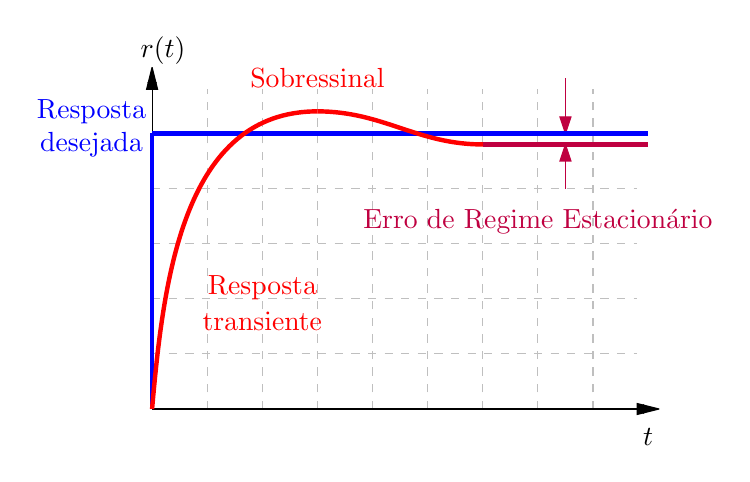
\begin{tikzpicture}[scale=0.70]
\draw [lightgray, dashed](0,0) grid (8.8,5.8);

\draw [->] (0,0) -- (9,0); 
\draw [fill] (0,6.2) -- (-0.1, 5.8) -- (0.1,5.8) -- (0,6.2);

\draw [->] (0,0) -- (0,6);
\draw [fill] (9.2,0) -- (8.8,0.1) -- (8.8,-0.1)--(9.2,0.0);

\draw [purple, ->] (7.5,4.0) -- (7.5,4.6); 
\draw [purple, fill] (7.5,4.8) -- (7.4,4.5) -- (7.6,4.5)--(7.5,4.8);

\draw [purple, ->] (7.5,6.0) -- (7.5,5.2); 
\draw [purple, fill] (7.5,5.0) -- (7.4,5.3) -- (7.6,5.3)--(7.5,5.0);

\node at (9.0,-0.5) {$t$};
\node at (0.2,6.5) {$r(t)$};

\draw [blue, ultra thick] (0.0,5.0) -- (9.0,5.0);
\draw [blue, ultra thick] (0.0,0.0) -- (0.0,5.0);

\draw [red, ultra thick] (0.0,0.0) to [out= 85, in=180] (3,5.4);
\draw [red, ultra thick] (3.0,5.4) to [out=  0, in=180] (6,4.8);

\draw [purple, ultra thick] (6,4.8) -- (9,4.8);

\node at (-1.1,5.4)[blue]{{Resposta}};
\node at (-1.1,4.8)[blue]{{desejada}};
\node at (2.0,2.2)[red]{{Resposta}};
\node at (2.0,1.6)[red]{{transiente}};
\node at (3.0,6.0)[red]{{Sobressinal}};
\node at (7.0,3.4)[purple]{{Erro de Regime Estacionário}};

\end{tikzpicture} 
\label{fig:funcaoResposta}

%{\small Fonte: \cite{dorf2011modern} }
\end{figure}



\end{frame}


%%%%%%%%%%%%%%%%%%%%%%%%%%%%%%%%%%%%%%% Diagrama de Blocos do Sistema em Malha Aberta
\begin{frame}{Diagrama de Blocos do Sistema em Malha Aberta \tiny \cite{Ogata}}

\begin{figure}[!htb]
\centering
%\caption{ Sistema de controle em malha aberta}
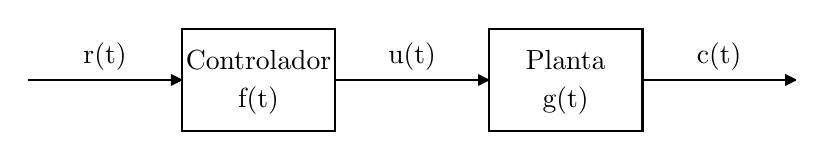
\begin{tikzpicture}[scale=0.65]
%\draw [lightgray](0,0) grid (15,2);
\draw (0,1) -- (3,1);
\draw [black, thick](3,0) rectangle (6, 2) ; 
\draw (6,1) -- (9,1);
\draw [black, thick](9,0) rectangle (12, 2) ; 
\draw (12,1) -- (15,1);

\draw [fill]( 3,1) -- ( 2.8, 1.1) -- ( 2.8,0.9) -- ( 3,1);
\draw [fill]( 9,1) -- ( 8.8, 1.1) -- ( 8.8,0.9) -- ( 9,1);
\draw [fill](15,1) -- (14.8, 1.1) -- (14.8,0.9) -- (15,1);

\node at ( 4.5, 1.4){Controlador};
\node at ( 4.5, 0.6){f(t)};
\node at (10.5, 1.4){Planta};
\node at (10.5, 0.6){g(t)};
\node [above] at ( 1.5,1){r(t)};
\node [above] at ( 7.5,1){u(t)};
\node [above] at (13.5,1){c(t)};
\end{tikzpicture}
%\label{fig:AcaoMalhaAberta}

%{\small Fonte: Próprio autor}
\end{figure}


Onde: 

\begin{itemize}
\item $r(t)$: Valor de Referência em rotações por segundo [rps];

\item $f(t)$: Controlador que converte rps em \% PWM para acionar o motor;

\item $u(t)$: Variável Manipulada é o valor percentual do PWM;

\item $g(t)$: Planta ou Processo formado pelo motor CC com o disco acoplado no eixo;

\item $c(t)$: Variável Controlada é a velocidade de rotação do eixo em rps.
\end{itemize}

\end{frame}



%%%%%%%%%%%%%%%%%%%%%%%%%%%%%%%%%%%%%%% Modelagem matemática
\begin{frame}{Modelagem matemática \tiny \cite{Ogata}}

\centering
$C(s) = \frac{K}{s+a} \frac{A}{s} \rightarrow \mathscr{L}^{-1} \to c(t) = \frac{K A}{a} (1 - e^{-at})$


\begin{figure}[!htb]
\centering
%\caption{Sistema de Primeira Ordem}
\subfloat[Sinal de entrada tipo degrau com amplitude A]{\label{fig:degrauA}
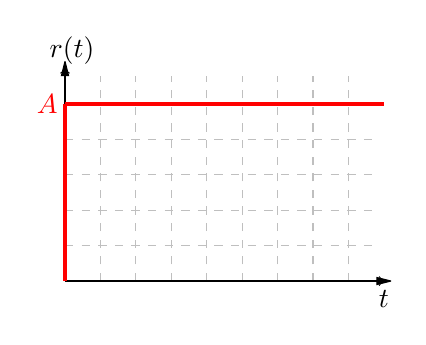
\begin{tikzpicture}[scale=0.45]
\draw [lightgray, dashed](0,0) grid (8.8,5.8);
\draw [->] (0,0) -- (9,0);
\draw [fill] (0,6.2) -- (-0.1, 5.8) -- (0.1,5.8) -- (0,6.2);
\draw [->] (0,0) -- (0,6);
\draw [fill] (9.2,0) -- (8.8,0.1) -- (8.8,-0.1)--(9.2,0.0);
\node at (9.0,-0.5) {$t$};
\node at (0.2,6.5) {$r(t)$};
\draw [red, ultra thick] (0.0,5.0) -- (9.0,5.0);
\draw [red, ultra thick] (0.0,0.0) -- (0.0,5.0);
\node at (-0.5,5.0)[red]{$A$};
\end{tikzpicture} }
\subfloat[Resposta transitória e regime de acomodação]{\label{fig:cRegime}
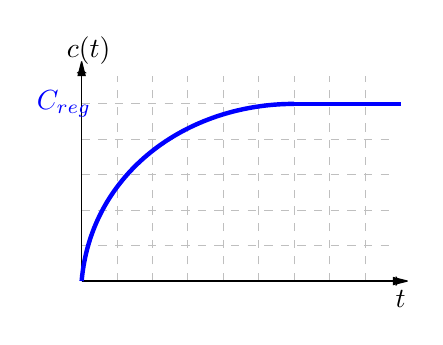
\begin{tikzpicture}[scale=0.45]
\draw [lightgray, dashed](0,0) grid (8.8,5.8);
\draw [->] (0,0) -- (9,0);
\draw [fill] (0,6.2) -- (-0.1, 5.8) -- (0.1,5.8) -- (0,6.2);
\draw [->] (0,0) -- (0,6);
\draw [fill] (9.2,0) -- (8.8,0.1) -- (8.8,-0.1)--(9.2,0.0);
\node at (9.0,-0.5) {$t$};
\node at (0.2,6.5) {$c(t)$};
\node at (-0.5,5.0)[blue]{$C_{reg}$};
\draw [blue, ultra thick] (0,0) to [out=85, in=180] (6,5);
\draw [blue, ultra thick] (6,5) -- (9,5);
\end{tikzpicture}}
%\label{fig:sistPrimeiraOrdem}

%{\small Fonte: Próprio autor}
\end{figure}


\end{frame}



%%%%%%%%%%%%%%%%%%%%%%%%%%%%%%%%%%%%%%% Modelagem matemática
\begin{frame}{Modelagem matemática \tiny \cite{Ogata}}

Tomando $t= \frac{1}{a} = a^{-1} = \tau$ para gerar um valor conhecido em $e^{-at}$, da Equação anterior temos:

\vspace{1cm}

$ c(a^-1) = \frac{KA}{a}(1-e^{-(a.a^{-1})}) = \frac{KA}{a}(1-e^{-1}) = \frac{KA}{a}.0,63 = 0,63 . C_{reg} $

\begin{figure}
\centering
%\caption{Constante de tempo}
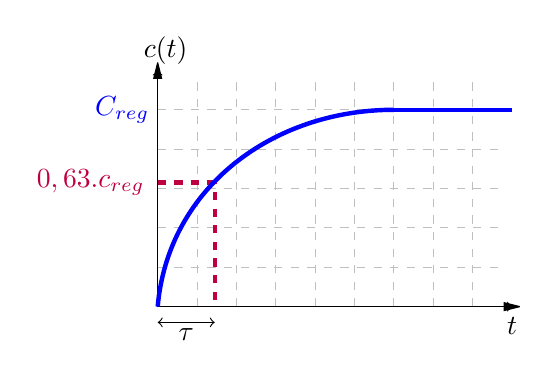
\begin{tikzpicture}[scale=0.50]
\draw [lightgray, dashed](0,0) grid (8.8,5.8);

\draw [->] (0,0) -- (9,0);
\draw [fill] (0,6.2) -- (-0.1, 5.8) -- (0.1,5.8) -- (0,6.2);
\draw [->] (0,0) -- (0,6);
\draw [fill] (9.2,0) -- (8.8,0.1) -- (8.8,-0.1)--(9.2,0.0);

\node at (9.0,-0.5) {$t$};
\node at (0.2,6.5) {$c(t)$};

\node at (-0.9,5.0)[blue]{$C_{reg}$};
\node at (-1.7,5.0*0.63)[purple]{$0,63.c_{reg}$};
\draw [purple, ultra thick, dashed] (0.0,5.0*0.63) -- (1.45,5.0*0.63)
						   -- (1.45,0.0);
\draw [blue, ultra thick] (0,0) to [out=85, in=180] (6,5);
\draw [blue, ultra thick] (6,5) -- (9,5);

\draw [<->] (0.0,-0.4) -- (1.45,-0.4); 
\node at (1.45/2,-0.7){$\tau$};

\end{tikzpicture}
%\label{fig:constTempo}

%{\small Fonte: Próprio autor}
\end{figure}


\end{frame}

%%%%%%%%%%%%%%%%%%%%%%%%%%%%%%%%%%%%%%% Ação de Controle em Malha Aberta
\begin{frame}{Ação de Controle em Malha Aberta}
Para $\tau = 2,5s $ calcula-se o polo da função:
$  a = \frac{1}{\tau} = \frac{1}{2,5} = 0,4 $
\vspace{-0.5cm}
\begin{figure}[!htb]
%\caption{Ação de Controle em Malha Aberta}
\center\includegraphics[scale=0.9]{./imagens/acaoMalhaAbertaTau.eps}
\label{fig:acaoMalhaAberTau}

%{\small Fonte: Próprio autor}
\end{figure}


\end{frame}


%%%%%%%%%%%%%%%%%%%%%%%%%%%%%%%%%%%%%%% Formato Canônico
\begin{frame}{Modelo do Sistema em Malha Aberta - Formato Canônico}

$  \frac{C(s)}{R(s)}=\frac{K}{s+a}=\frac{0,4}{s+0,4} $
\hspace{1cm}
$\frac{C(s)}{R(s)} = \frac{1}{\tau s+1} = \frac{1}{2,5 s+1} = g(t)$

\vspace{-0.5cm}
\begin{figure}[!htb]
%\caption{Ação de Controle em Malha Aberta}
\center\includegraphics[scale=0.9]{./imagens/acaoMalhaAbertaTau.eps}
\label{fig:acaoMalhaAberTau}

%{\small Fonte: Próprio autor}
\end{figure}


\end{frame}



%%%%%%%%%%%%%%%%%%%%%%%%%%%%%%%%%%%%%%% Qualidade do Modelo
\begin{frame}{Qualidade do Modelo}
Erro Relativo Percentual

\begin{equation}
 \% erro = \frac{100}{N} . \sum_{n = 0,00}^{n=22,40} {\frac{| \text{\emph{r[n]}} -\text{\emph{c[n]}} |}{\text{\emph{r[n]}}} } 
\end{equation}

Onde:

\setlength{\parindent}{2cm}
r : valor real; 

c : valor calculado;

n : número da amostra aquisitada;

N : número total de amostras.


\end{frame}



%%%%%%%%%%%%%%%%%%%%%%%%%%%%%%%%%%%%%%% Qualidade do Modelo
\begin{frame}{Qualidade do Modelo}

\begin{table}[h]
\centering
\caption{Erro Relativo Percentual para intervalos determinados por $\tau$ }
\label{tab:ErroModeloTau}

\begin{tabular}{c|c}
\hline
Intervalo de amostras  &  erro médio relativo \\ \hline
\hline
%0 a 1 $\tau$ & 83,40 \% \\ \hline
1 a 2 $\tau$ &  3,16 \% \\ \hline
2 a 3 $\tau$ &  3,38 \% \\ \hline
3 a 4 $\tau$ &  2,00 \% \\ \hline
4 a 5 $\tau$ &  2,29 \% \\ \hline
$>$ 5 $\tau$ &  0,82 \% \\ \hline
\end{tabular}

%{\vspace{0.2cm} \small Fonte: Próprio autor}
\end{table}


\end{frame}

